\documentclass{article}

\usepackage{Sweave}
\begin{document}
\Sconcordance{concordance:04_analysis.tex:04_analysis.Rnw:%
1 2 1 1 0 20 1}




\section{Analysis}

\subsection{Exploratory Data Analysis}
Before building our model, we first wanted to understand the data that we were building our model on. Below, I've hsown the summary statistics for the quantitative variables as well as histograms for ACT scores, SAT scores, and graduation rates. 

\input{quantitative_summary, file = '../../data/eda.txt'}
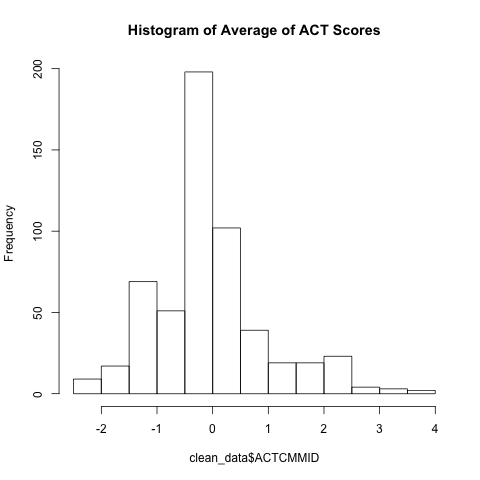
\includegraphics{../../images/histogram_ACT_avg.png}
The maximum score for the ACT is 36.
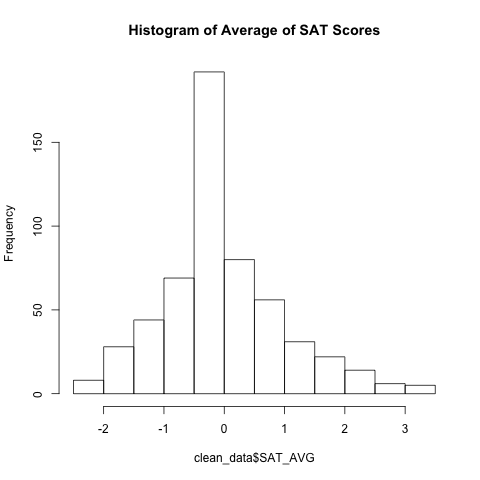
\includegraphics{../../images/histogram_SAT_avg.png}
The maximum score for the SAT is 2400.
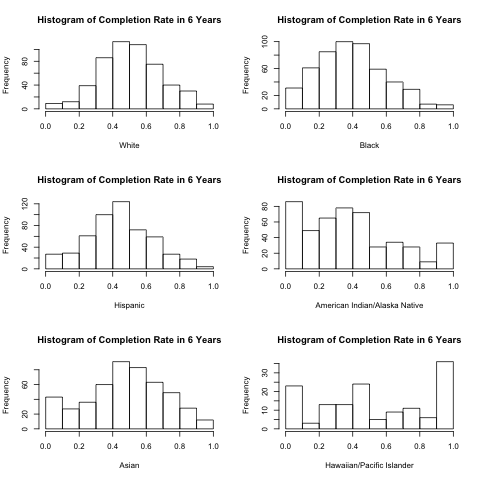
\includegraphics{../../images/histogram_race_completion}
The histogram above depics graduation rates for each ethnicity. 

\subsection{Variable Selection Methods}

\end{document}
